\documentclass[10pt,twocolumn]{article}

% use the oxycomps style file
\usepackage{oxycomps}

% usage: \fixme[comments describing issue]{text to be fixed}
% define \fixme as not doing anything special
\newcommand{\fixme}[2][]{#2}
% overwrite it so it shows up as red
\renewcommand{\fixme}[2][]{\textcolor{red}{#2}}
% overwrite it again so related text shows as footnotes
%\renewcommand{\fixme}[2][]{\textcolor{red}{#2\footnote{#1}}}

% read references.bib for the bibtex data
\bibliography{references}

% include metadata in the generated pdf file
\pdfinfo{
    /Title (The Foxglove Handheld Game Console)
    /Author (Lavender Perry)
}

% set the title and author information
% TODO: addition to title that says what it is
% like maybe --
% Foxglove: A handheld game console with emphasis on hacking
% or --
% Foxglove: Using a video game framework to create a handheld game console
% idk im not that worried about it right now
% this is just how ive seen other comps formatted
\title{The Foxglove Handheld Game Console}
\author{Lavender Perry}
\affiliation{Occidental College}
\email{lperry@oxy.edu}

\begin{document}

\maketitle

\section{Introduction and Problem Context}

Many game consoles, in particular older game consoles, have been hacked by
programmers to support homebrew development. Homebrew is a console application
made by an individual or group of individuals who do not have access to the
official tools provided by the console manufacturers. Another similar way for
individuals to make games for a console is ROM hacking, which is modifying
an existing game for the console. The term "hacking" in general can mean many
things, but the meaning I use is modifying a system to benefit the user, in a
way that resists the system's design.

ROM hacking and homebrewing allow
individuals to express themselves and learn about computers on a platform they
enjoy \cite{kacmarcik_introducing_2009}. More importantly, hacking of any
system, including games and consoles, helps marginalized people, including
disabled people, access these technologies and change systems that exclude them
better than a one size fits all approach to design \cite{hamraie_crip_2019}.
Hacking and remixing are important tools for self expression and protest,
particularly for people underrepresented in computer science, gaming, and
mainstream technology design.

Despite, or because of, the benefits of homebrewing and ROM hacking, few game
consoles facilitate homebrewing, and none facilitate ROM hacking. Many
handhelds, and systems in general, do not support hacking due to the political
and economic interests of the manufacturers not aligning with the users. The
business model of console manufacturers relies on restricting game and app
development to those who pay. Many ways an individual can hack, of systems
including game consoles, medical devices, or physical arcitecture, are illegal.
However, restricting the software through technical measures and law
closes the advantages of homebrew and indie
game development to highly technical users who can risk getting arrested.
As shown by the Nintendo Switch, a console's modding community
can become an exclusionary and elitist space, gatekeeping anyone who does not
have the time or resources to learn to mod, or anyone who can not afford to risk
breaking their console.
It can enforce the hegemony it should stand in opposition to, and fails the
exact people that have the most to gain from it \cite{brown_why_2022}.

My project is Foxglove, a handheld game console inspired by console hackers and
homebrewers. The console is designed to be opinionated and reflect my own ways
of playing games, yet encourage and facilitate others remixing and modifying it
as much as possible. It attempts to give users the tools to become designers of
the console and games on it, and share their modifications with others. My goal
is to build a world in the console while encouraging others to hack, build
and re-build their own, inviting users to design with and against me. I do so
to answer the question of if creating a game console that is easier to modify
will foster a more inclusive and supportive community, particularly for people
new to console modding.

\section{Technical Background}

These are the technical terms and concepts that are relevant to my project.

\subsection{Modding}

Modding, short for modifying, is taking a game or software and changing it.
Typically, this is done to add features or present a different ideal of how the
software should function, often in a way that serves the user and that the
original creator of the software did not anticipate. A large amount of my
project revolves around the idea of modding, and the rest of the terms in this
technical background are all related to it in some way.

\subsection{Code Injection}

Code injection is the process of making a software load and run third party
code. Injecting code is typically how modding is accomplished, and therefore
allows many of the practices discussed in this project to occur. Sometimes this
is accomplished by exploitable bugs in the software itself, while other times,
and in my project, it is accomplished by manipulating the environment in which
the software runs.

\subsection{Patches}

A patch describes how source code changes from one state to the next. Patches
function as instructions for how to apply source code changes, and are
especially useful for modding. Often, a modding API allowing users to inject
their code into software will take patches as input to specify what code should
be injected. Patches are commonly used in ROM hacking, as explained in the
following subsection.

\subsection{ROM Hacking}

ROM hacking is a specific type of modding targeted at console games.
Most console games are stored in read-only memory, or ROM.
This is typically binary data that is difficult to modify,
and is not intended to be copied or edited.
ROM hacking is the practice of copying and modifying the ROM to
change aspects of the game, such as art or text.
A ROM hack is the resulting game made from this practice.
Because a ROM hack relies on data from the original ROM,
which is often illegal to redistribute even in modified form,
ROM hacks are typically distributed as patches to the original ROM.
To play the ROM hack, users will use a tool called a ROM patcher to reconstruct
the modified ROM from the original ROM and the patches.
Similarly to a ROM patcher, my project may use a patch format to provide a
game modification system. Unlike ROM hacking, the game files will exist
as Lua source code, which is easier to read, copy, and modify.
More information about my modding and patching system is in section 4.

\subsection{Homebrew}

Homebrewing is similar to ROM hacking, but does not involve any modification
of video games. Instead, the process involves developing a game or application
from scratch, using community provided development tools. Many game consoles
have official development tools available to anyone, which I will elaborate on
in section 3. For consoles without official and available development tools, or
that disallow third party development, homebrewing is a useful practice.

\section{Prior Work}

There are multiple studies as well as other projects that are relevant to
Foxglove, which I discuss and categorize here.

\subsection{Accessibility}

One of the goals my project has is to support game accessibility without being
overly prescriptive, as accessibility needs vary significantly between
individuals. Although some bias towards certain needs is inevitable, design
recommendations such as those proposed by Martinez et al. after interviewing
disabled gamers may help in creating a gameplay system which supports gamers in
finding and adapting games to work for them. Recommendations which are within
the scope of this project include providing mechanisms for the player to
customize the game as well as documenting these mechanisms in an easily
discoverable place \cite{martinez_playing_2024}. More information on how I
integrate these design recommendations are in section 4.

\subsection{Cheap and Low Power Handhelds}

ENGAGE is a Game Boy compatable handheld console that works
without a battery.
Instead, it uses a small solar panel as well as buttons that harvest energy
from the gamer's actions to power the device.
What I found most interesting is the power saving methods they used,
which I may adopt for my own device.
Although some methods had drawbacks to them, such as using a non-backlit screen,
one that had very little drawbacks was attaching an external FRAM device.
Another interesting aspect of the ENGAGE is it
reads the memory values of the Game Boy game
and stores them to reload them
when the console loses and regains power \cite{de_winkel_battery-free_2020}.
I plan to introduce a general purpose modding API into my handheld that
gives access to the modded game's memory, although at a higher level.

\subsection{Controllers}

Many handheld game consoles do not prioritize third party controller support
in their design, in part due to their small, portable form factors.
However, many people create their own controllers and may wish
to use them with the handhelds. A common practice is using everyday objects, to
lower both the financial cost and environmental impact of
creating the controllers. An example is work by Pokorny et al., which uses
microcontrollers and common household objects to create controllers designed for
existing games \cite{pokorny_bin_2023}. Kits such as Makey Makey additionally
open the process to individuals with no background in electronics
\cite{collective_makey_2012}. See section 4 for how my console will be designed
to support these controllers.

\subsection{Development and Modding Platforms}

Although some game consoles close off development to users, requiring them to
create homebrew, others, especially more recently, are designed to allow users
to develop for them. One such example is PlayDate. It provides developer tools
and explicitly encourages independent developers to make games for the platform.
These tools additionally take steps to encourage transparent, accessible games
by allowing developers to specify content warnings in the game metadata
\cite{inc_inside_nodate}.

Providing an open development platform for a game console is one way to make
creation for the console easier. Additionally, there are efforts to lower the
technical barrier to creating homebrew for existing consoles, made by and for
users of the console.
One such example is LÖVE Potion, a port of the LÖVE video
game framework to Nintendo consoles, including the 3DS, Wii U, and Switch
\cite{noauthor_lovebrewlovepotion_2025}.
LÖVE Potion allows users to make games
for these consoles without having to use systems programming languages such as
C, and gives them high level functions and abstractions to make the process
significantly more beginner friendly. Because LÖVE
has been successfully adapted
to game consoles, and it is flexible enough to adapt to my own console, I am
utilizing it for my development platform. Modding tools for LÖVE,
such as
Lovely, may also be used to provide tools for modding on the console.
Lovely is a library that, when loaded alongside LÖVE,
allows for Lua code injection into a
LÖVE game. Although primarily used to mod Balatro,
it should work for any other
game made with the LÖVE framework.
\cite{green_ethangreen-devlovely-injector_2025}. More information on how I use
LÖVE and how I plan to use Lovely for this project
is in section 4.

\subsection{Launchers}

One of the core components of any game console is a menu to access the games and
other applications on the console. Commonly called launchers, an example of one
that integrates the LÖVE framework is Love Launcher
\cite{noauthor_glitchapplovelauncher_nodate}. Although it does a lot of things
that I can incorporate into my launcher, it is not suitable to use with
my handheld. Most significantly, it is not designed with the handheld form
factor in mind. In section 4 I will explain what aspects of this launcher I take
inspiration from, and what I choose to do differently from it.

\section{Methods}

Foxglove consists of multiple components:
the physical console hardware, the
game launcher, and the operating system. These components integrate with each
other to create a fully functional game console.

\subsection{Launcher}

The launcher (available on GitHub
\cite{perry_lavenderperryfoxglove-launcher_2025})
handles listing games to the user, managing console settings, and
running console games. Similarly to Love Launcher,
it is built using the LÖVE
framework and runs games built on that same framework. The primary architectural
difference between Foxglove's launcher and
Love Launcher is, while Love Launcher
creates a new process and starts up the framework whenever a game is launched,
Foxglove's launcher uses the existing process to run the game,
allowing the game
to take control over the process that the launcher is running in
\cite{noauthor_glitchapplovelauncher_nodate}. I chose this approach for two
reasons. My primary reason is that the console draws all of its graphics using
low level Linux graphic APIs, and it is much simpler to have one process
interfacing with these APIs than it is to have multiple processes. The other
reason is I can easily modify the framework by running the game's code in
specific ways. One way I use this to my advantage is by wrapping the game's exit
handling code to exit back to the launcher instead of quitting entirely. In the
future, I hope to modify the games in a way that introduces a modding API,
elaborated upon in the next subsection.

\begin{figure}[!htb]
    \centering
    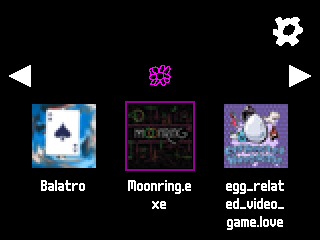
\includegraphics[width=.95\linewidth]{launcher.png}
    \caption{
        A screenshot of the launcher, showing a menu for selecting games.
    }
    \label{fig:launcher}
\end{figure}

For the UI, the user scrolls through the games, showing three at a time on the
screen. It is inspired by other game consoles, such as the Nintendo Switch, that
scroll through games in a similar way \cite{noauthor_nintendo_nodate}. The
graphics of the menu currently use only three colors, so that they can be
customized without overwhelming the user with large amounts of colors to change.
I also show images for each of the games, which are currently specified in a
seperate directory from them. In the final version, the path to the image will
be specified by the game metadata, described in subsection 4.4.

\subsection{Modding API}

The modding API may integrate with tools such as Lovely
to allow for direct
source code modification of games. Using Lovely's patch format,
the user will be
able to specify code to inject into the source of a game
\cite{green_ethangreen-devlovely-injector_2025}. This allows for large
amounts of flexibility in modding games, as third party code may modify anything
the user would like, including implementing an entirely different game on top of
an existing one.

Another type of modding API I may choose to implement is a system built around
callback functions. As my current game launcher already has access to the
process in which the game is running, it can call other functions before or
after calling specific functions the running game defined. By calling functions
defined by a mod in specific situations, I can implement a callback-based
modding API.

One advantage of a callback-based modding API over direct source code
modification through patches is that the user does not have to reference the
game's source code as much. Instead of thinking about their changes based on
what position in the original source code they will take place at, the user can
think about their changes based on what situation they will be executed at. This
may facilitate modding better, especially for users unfamiliar with reading
source code. A callback-based system may also be easier for users because there
is no patch format to learn. Instead, callbacks are specified simply by defining
functions, so there is nothing extra to learn in addition to the coding skills
necessary to mod games already. Another advantage to a callback-based system is
it decreases the chance of issues when applying multiple mods to the same game.
If multiple people make a mod for the same game, their source code may overwrite
each other in a patch-based system. In a callback-based system, it is easier to
ensure compatability between mods, as all mod functions are called separately
from each other and can not overwrite each other.

However, a patch-based system has many advantages over a callback-based system.
First, it is much more flexible. While a callback-based system limits modders to
injecting their code only where I have created a callback, a patch-based system
allows modders to inject their code anywhere. Additionally, a callback-based
system may be created on top of a patch-based system, but a patch-based system
can not be created on top of a callback-based system. Another reason to prefer a
patch-based system is I can use Lovely for part of it
instead of needing to
implement the entire thing from scratch. This also partially mitigates the
disadvantage of needing to learn a patch format, because users may already know
Lovely's format,
or may choose to use their knowledge of the format for modding
outside the context of Foxglove.

\subsection{General Customization}

Although customization is possible through the modding API, options should be
provided for the user that do not require console modding. The primary
categories for customization I am thinking of right now are color and font
customization. Color customization may
include presets such as light, dark, low contrast, and high contrast, as well as
allowing users to specify each of the three colors manually. The presets are
available to avoid overwhelming the user with choices, while the manual option
for setting colors is available for users who prefer maximum control. For font
customization, including fonts shown to be readable for people both with and
without dyslexia, such as Arial, Computer Modern, Courier, and Helvetica may
improve the usability of the UI \cite{rello_effect_2016}. Font size and style
(regular, italic, bold) are other aspects of fonts that may be customizable.

\subsection{Integrated and Custom Controls}

The main control scheme I am considering for
Foxglove consists of 4 to 7
buttons. This lower than average amount of buttons is in the range of an older
console, such as the Game Boy with 8 buttons,
when the directional pad, or D-pad,
is counted as 4 \cite{de_winkel_battery-free_2020}.
One reason to choose this amount is to
reduce the learning curve for using the controls. With less possible inputs,
there are less motions for the player to learn and do, which may also make
Foxglove accessible to people who struggle with many possible inputs.
Another
advantage to having less buttons is making the built in controls and custom
controllers for Foxglove is easier.
For both myself while making the console and
for others while creating controllers for the console, it requires less hardware
and makes assembly simpler. Users making custom controllers will have more
options in terms of form factor, as they have less inputs they need to map to.
The integrated controls on the console will likely have 4 of its buttons, or
inputs, be satisfied by a D-pad, so that games may take advantage of a
directional element.

Another design element of the integrated control scheme which I considered
is putting the buttons on the back of the console. Doing so has the benefit of
making custom controllers feel better integrated into the console, as you can
not see the integrated controls while using the console. It also allows for
users to control the console with the rest of their fingers, rather than
their thumbs, which may be preferable to some. One drawback of having controls
on the back is that setting the console down on a table would possibly press all
the buttons. A way to avoid this would be to not accept inputs from integrated
controls whenever an external controller is plugged in. However, it would also
likely be easier to put the controls on the front and make custom controllers
feel more integrated another way, such as allowing the symbols used to represent
buttons on the controller to change based on the controller plugged in.

\subsection{Game Metadata}

Games will be able to define metadata, which tells the console how to handle the
game. It will be similar to PlayDate's metadata definition system in that it
will work using a file at the root directory \cite{inc_inside_nodate}. This file
will likely be in TOML, which is already used by Lovely
\cite{green_ethangreen-devlovely-injector_2025}. Using a standard format
decreases the amount of work I need to do to parse it and increases the chance a
user has already learned the format. Metadata will include the game title,
author(s), version, a path to an icon to represent the game,
a list of accessibility features the game supports, and a list of content
warnings that apply to the game. All of these fields will be displayed by the
launcher in some way.

%The next steps for game functionality
%are allowing users to easily install games
%and providing tools to modify the games. Installation may be done through
%external storage such as USB drives or SD cards that are inserted into the
%console and copied to the console storage. Modification of games may use a
%pattern-based patch system such as Lovely}
%\cite{green_ethangreen-devlovely-injector_2025}. Alternatively, callbacks
%injected by the launcher may be used by making the launcher load custom code
%specified by the modifications.

\section{Evaluation Metrics}

Although the project is still at an early stage, evaluation shows that the
launcher is on the right track for meeting goals of functionality
(being able to run games) and aesthetics (looking pretty). More work is needed
before any positive judgement can be made on ease of use (users can use the
launcher without guidance), customizability (launcher and games can be
modified to fit user preferences), and integration (launcher works with the
other components). Only the launcher is evaluated here, as work on other
components has not been started yet. A discussion of future metrics is present
in subsection 5.3.

\subsection{Testing With Games}

To ensure the launcher can handle a reasonable variety of games, I tested
multiple games made with the LÖVE framework.
Games could all be listed in the UI
and launched. Any game that relies on mouse input does not work when the
launcher is ran on the low level graphics APIs the console uses. However, this
is an acceptable shortcoming, as the handheld game console will not have a
mouse. Other than that, all games are listed, launch, and run as expected.

\subsection{User Testing}

As the launcher is not complete yet, it has only had one user tester so far,
with more being planned as development continues. The tester was able to
navigate the UI with some guidance. The need for guidance should decrease when
the launcher is on the actual console, because the control scheme will be more
apparent by the physical design, but this is still an issue to consider in
future testing. The tester liked the aesthetics of the UI as well. When asked
if there are any aspects of the UI the tester would want to customize, they
responded that they would appreciate a light mode, where the UI has a light
background with a dark foreground. Another item of feedback the tester gave is
there should be the ability to customize the font. Customization options of the
UI have not been implemented yet, but the tester's feedback has revealed color
and font customization as a viable starting point. Ideas for font and color
customization are elaborated upon in the previous section.

\subsection{Future Metrics}

To determine if Foxglove reaches the goal of being easy to mod and
extend, I intend to perform more user testing, but with a primary focus on ease
of developing games for and modding of the console. Testers will be primarily
individuals with little to no experience with computer science, to avoid
creating a system that is easy for computer scientists,
but difficult for others. Additionally, testing on a wide variety of users must
occur see how successfully Foxglove meets goals of accessibility, and
for which users it meets or fails those goals.

Additionally, I may attempt to teach an informal class
class on developing and modding games on Foxglove. The goal of this is
to see if Foxglove is easy enough to teach to others with no
experience, as well as to see what kind of community Foxglove can help
build through this setting. The main issue with this type of evaluation is that
failures in the class may be due to my own incompetency as a teacher, rather
than any failures with the project. An alternative option is to get someone else
to do it, but that is much more work than I would feel comfortable asking
someone else to do.

Alternatively, to evaluate the community building goals of my project, I can
attempt to spread the project and see what community results from it. This would
be primarily on the internet, as most other console modding communities are
\cite{brown_why_2022}. Forums and chatrooms that surround similar topics to my
game console and encourage sharing projects are ideal spaces. If promotion of
Foxglove is done in a similar space to console modding projects and
communities, it should be easier to compare what occurs to those other
communities. The main issue with this idea is that communities take time to
develop, so it would likely take past the due date for any conclusions to be
made about this evaluation. It is likely best left as future work, as is the
previous idea.

\section{Results and Discussion}

As shown by testing, the game launcher was a successful first step towards my
project. My most significant next steps include getting the launcher to run on
hardware more similar to the eventual final project, as well as beginning to
implement modding APIs. One potential necessary technical change to the launcher
would be to give it more control over the LÖVE
game framework environment that
it runs in. This would require either making the launcher itself be a modified
version of
LÖVE, or creating a seperate application that uses the LÖVE
library.
The process of doing either of these things may require rewriting some or all of
the existing code from Lua to C++. A rewrite such as this one should be done as
early as possible to avoid having to rewrite more code than necessary.

\section{Ethical Considerations}

The ethics of my project mainly revolve around the fact that I am building
for the world that I wish existed, not the one we currently live in. Although my
project could potentially get more people into art, video games, and computer
science, the issues excluding people from doing those things are at least
partially community and societal, rather than technological.
I explore how making
something easier is not always the solution, consider the role of an
individual's lack of free time in creating an access barrier, and explain the
issues involved in making a hardware-based project such as my own. Despite the
ethical issues arising from my project, I believe it is still worthwhile to
pursue.

\subsection{Difficulty}

One important consideration is if the project will, rather than encouraging
users to hack and expand on game consoles, have the opposite effect.
Goode and Cruise argue that a significant motivating factor for people to remove
copy protection from software is the difficulty in doing so, where the
individual removing the copy protection seeks a personal challenge
\cite{goode_what_2006}. Although this could be considered hacking, it is not the
type of hacking I am interested in for the purposes of this project. However, it
is likely there is some crossover, in that people making and modifying games and
applications for game consoles are motivated, in part or entirely, by the
difficulty of it. Motivation by challenge is likely not a quality exclusive to
any specific subset of individuals, so applying it to console modding is
appropriate. Therefore, making the process of creating and modifying for my
console easier may discourage, rather than encourage others from doing so.

However, there are other motivations to hack which must be considered.
Brown et al. respond to Goode and Cruise's argument with an alternate view of
why users hack, which emphasizes a difference in interests between the users and
the designers, or the organization dictating what the designers may do
\cite{brown_why_2022}. At first glance, this implies a failure on the designer's
part, yet a better way to view this is through bad design being an individual
judgement that varies from person to person. Therefore, it is possible for users
to still want to modify a project even if it is not maliciously designed.
Even if some users are put off by it being too easy, a significant amount who
were already turned away by it being too difficult will be interested. It should
also be possible for users to scale up the difficulty level depending on what
they make as needed.

\subsection{Accessibility / "Good" Design}

Encouraging modification may help individuals overcome design issues that affect
them, however using it as a solution for every design issue is lazy and requires
the user to do too much labor. If the user has to do too much work to make the
console accessible to them, they may decide it is not worth the trouble, such as
in the case of some of the disabled gamers polled by Martinez et al.
\cite{martinez_playing_2024}. Frequent testing with as wide a variety of people
that my intended audience consists of is necessary to catch design issues that
can be mitigated without too negative a tradeoff, and re-evaluating who my
audience is as I complete the project is also important. Without paying
attention to these things, preventable accessibility issues may occur.

\subsection{Time}

Another consideration is under our past and current hegemonic society, time is a
limited, commodified resource. Fellner defines the commodification of time by
defining a set of motivations for how people use their time, which are power,
playfulness, meaning, and belonging. The process of commodifying time involves
increasing the percieved importance of power at the cost of anything else. This
means people often have to devote all their time to capitalist labor and do not
have time to create or enjoy art \cite{fellner_value_2017}. Having time for
things like this game console is a luxury that is most available to individuals
least impacted by systematic oppression. I'm not exactly sure how to mitigate
these issues, but they're important to think about before implementing features
that require the user to have lots of free time. It may also be another point in
favor of making creating and modding for the console easier, as the more
difficult it is, the more time it will take to learn how to do it.

\subsection{Hardware}

As this project is a game console, a significant part of it will be
hardware-based. This makes the project harder to reproduce, as anyone seeking to
reproduce it will have to purchase hardware. Mining of materials to use in that
hardware involve inhumane labor practices and exploitation, especially of
communities in the Global South. This extractive, colonial process also
wrecklessly destroys the environment for profit. However, all computer
technologies -- including my project, including any devices for personal or
educational use, and including any devices used to raise awareness about and
protest against this issue -- all rely on the materials mined through this
process, and therefore are complicit in the problem. When raising these issues,
de Castro Leal et al. do not suggest abandoning technology altogether, instead
raising questions for computer scientists to consider when building projects and
conducting their research. Many of these questions encourage de-emphasizing
innovation in exchange for slower, more thoughtful creation and use of
technology \cite{de_castro_leal_into_2021}.

In considering these questions, I have primarily focused on creating an
imperfect but more sustainable than average game console. It is useful to think
of my project not as the single final deliverable, but as many copies of it
distributed on a large scale, as that is what would likely do the most harm.
Extra peripherals will be minimized to avoid relying even more on unethically
produced materials. Hardware performance will be neglected entirely to
discourage the industry's unsustainable obsession with recreating hardware to
achieve the fastest performance possible, thereby furthering the disregard for
sustainability and human rights. All software made for this project will run on
other hardware, albeit with potential usability compromizes on those platforms,
to avoid the requirement to rebuild the hardware in order to experience the
project. Despite these measures, I, along with most other computer scientists,
am complicit in this harmful process. No amount of consideration on an
individual level will solve these systemic issues of imperialist exploitation,
yet it is critical to attempt to address the ethics anyways, especially in
projects like this one.

\section{Timeline}

An initial idea for the timeline of my project is as follows:

\begin{itemize}
    \item June
        \begin{itemize}
            \item Begin prototyping hardware
        \end{itemize}
    \item July
        \begin{itemize}
            \item Obtain components for the hardware
        \end{itemize}
    \item August
        \begin{itemize}
            \item Week 1-2: Work on the modding APIs and solidify the intended
                  game development process
            \item Week 3-4: 3D print a case for the hardware components
                  based on my prototype and begin constructing the hardware
        \end{itemize}
    \item September
        \begin{itemize}
            \item Week 1-2: Determine the most appropriate control scheme for
                  the console and implement it
            \item Week 3-4: Make the Linux environment that runs the game
                  launcher and put it on the hardware
        \end{itemize}
    \item October
        \begin{itemize}
            \item Week 1-2: Work on a system to install games from USB media
            \item Week 3-4: Finalize the documentation for the project, writing
                  less technical tutorials in addition to refining all technical
                  documentation
        \end{itemize}
    \item November
        \begin{itemize}
            \item Week 1-2: Evaluate the success of the project with more
                  focused user testing
            \item Week 3-4: Work on graphics, aesthetics and poster
        \end{itemize}
    \item December
        \begin{itemize}
            \item Week 1-2: Refine project, update poster if needed
            \item Week 3-4: Last minute changes, submit the project
        \end{itemize}
\end{itemize}

\printbibliography

\appendix

\clearpage

\onecolumn

\end{document}
